\documentclass[12pt]{article}
\usepackage{worksheet-common}
\usetikzlibrary{arrows.meta,calc}

% Written HW 5 -- Ohm's law, the junction & loop rules, series & parallel
% resistors (Knight 27.5, 28.1-28.4, 28.6). Due Wed Oct 7.
% Section 1 = required (9 problems, 2 pts each = 18 pts).
% Section 2 = extra credit (9 problems, 1 pt each, up to +9 pts).
% All ideal batteries (r=0) -- multi-battery loop problems are intentionally
% not included this time.

\newcommand{\battv}[1]{% vertical battery symbol centered at (#1)
  % explicit leads, guaranteeing the plates connect to the rest of the
  % loop even if the background wire doesn't render cleanly behind them
  \draw[line width=0.7pt] ($(#1)+(0,0.55)$) -- ($(#1)+(0,0.12)$);
  \draw[line width=0.7pt] ($(#1)+(0,-0.12)$) -- ($(#1)+(0,-0.55)$);
  \draw[line width=1.1pt] ($(#1)+(-0.35,0.12)$) -- ($(#1)+(0.35,0.12)$);
  \draw[line width=2.4pt] ($(#1)+(-0.2,-0.12)$) -- ($(#1)+(0.2,-0.12)$);
  \node[scale=0.75] at ($(#1)+(0.6,0.12)$) {$+$};
  \node[scale=0.75] at ($(#1)+(0.6,-0.12)$) {$-$};
}
\newcommand{\reszig}[1]{% horizontal resistor zigzag centered at (#1)
  \fill[white] ($(#1)+(-0.65,-0.32)$) rectangle ($(#1)+(0.65,0.32)$);
  \draw ($(#1)+(-0.6,0)$)
    -- ($(#1)+(-0.42,0.22)$) -- ($(#1)+(-0.24,-0.22)$)
    -- ($(#1)+(-0.06,0.22)$) -- ($(#1)+(0.12,-0.22)$)
    -- ($(#1)+(0.3,0.22)$) -- ($(#1)+(0.48,-0.22)$)
    -- ($(#1)+(0.6,0)$);
}
% \jarrow{angle}{in|out}{label} -- a labeled arrow into/out of a junction
% dot at the origin.
\newcommand{\jarrow}[3]{%
  \ifstrequal{#2}{in}{%
    \draw[-{Stealth[length=3mm]}, line width=1pt] (#1:1.5) -- (0,0);
  }{%
    \draw[-{Stealth[length=3mm]}, line width=1pt] (0,0) -- (#1:1.5);
  }%
  \node[scale=0.85] at (#1:1.95) {#3};%
}

\begin{document}

\worksheettitle{Written HW 5 --- Circuits I}

\noindent Ohm's law, the junction rule, the loop rule, and series \&
parallel resistors. \textbf{Section 1 is required: 9 problems, 2 points
each (18 points total).} \textbf{Section 2 is extra credit: 9 problems, 1
point each (up to 9 extra points).} Every battery below is ideal
($r=0$). Show your work.

%============================================================
\partsec{1}{Required --- 2 points each}

\prob A resistor has resistance $R=25\ \Omega$. A voltmeter placed across
it reads $\Delta V=15$ V. What current flows through the resistor?

\worksp{sm}

\prob Three wires meet at the junction shown below. Find the current $I$
leaving the junction.

\begin{center}
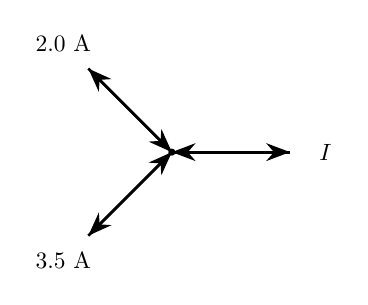
\begin{tikzpicture}[scale=1.0]
  \fill (0,0) circle (1.3pt);
  \jarrow{135}{in}{$2.0$ A}
  \jarrow{225}{in}{$3.5$ A}
  \jarrow{0}{out}{$I$}
\end{tikzpicture}
\end{center}

\worksp{sm}

\prob Four wires meet at the junction shown below. Find the unknown
current $I$.

\begin{center}
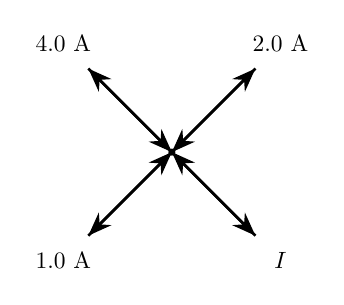
\begin{tikzpicture}[scale=1.0]
  \fill (0,0) circle (1.3pt);
  \jarrow{135}{in}{$4.0$ A}
  \jarrow{225}{in}{$1.0$ A}
  \jarrow{45}{out}{$2.0$ A}
  \jarrow{315}{out}{$I$}
\end{tikzpicture}
\end{center}

\worksp{sm}

\prob The single-loop circuit below has a battery with $\varepsilon=20$ V
and two resistors in series. A voltmeter reads $\Delta V_1=12$ V across
the first resistor. Find $\Delta V_2$ across the second.

\begin{center}
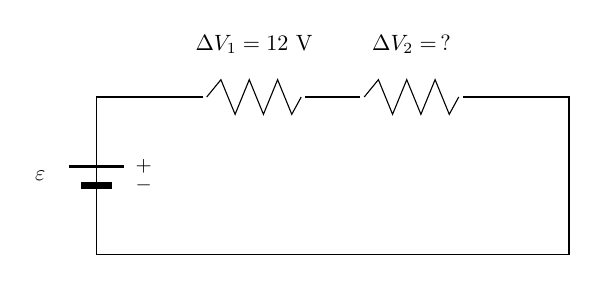
\begin{tikzpicture}[x=1cm,y=1cm]
  \draw (0,0) -- (0,2) -- (6,2) -- (6,0) -- cycle;
  \battv{0,1} \node[scale=0.8, anchor=east] at (-0.55,1) {$\varepsilon$};
  \reszig{2,2} \node[scale=0.8, anchor=south] at (2,2.45) {$\Delta V_1=12$ V};
  \reszig{4,2} \node[scale=0.8, anchor=south] at (4,2.45) {$\Delta V_2=\,?$};
\end{tikzpicture}
\end{center}

\worksp{sm}

\prob Same idea, different numbers: a single loop has $\varepsilon=24$ V
and two series resistors. $\Delta V_1=9.0$ V. Find $\Delta V_2$.

\worksp{sm}

\prob Two resistors, $R_1=4.0\ \Omega$ and $R_2=8.0\ \Omega$, are in
series with a battery of $\varepsilon=18$ V.

\begin{center}
\begin{tikzpicture}[x=1cm,y=1cm]
  \draw (0,0) -- (0,2) -- (6,2) -- (6,0) -- cycle;
  \battv{0,1} \node[scale=0.8, anchor=east] at (-0.55,1) {$\varepsilon$};
  \reszig{2,2} \node[scale=0.8, anchor=south] at (2,2.45) {$R_1$};
  \reszig{4,2} \node[scale=0.8, anchor=south] at (4,2.45) {$R_2$};
\end{tikzpicture}
\end{center}

\noindent Find (a) the equivalent resistance, and (b) the current
supplied by the battery.

\worksp{md}

\prob Three resistors, $R_1=2.0\ \Omega$, $R_2=3.0\ \Omega$, and
$R_3=5.0\ \Omega$, are in series with a battery of $\varepsilon=20$ V.

\begin{center}
\begin{tikzpicture}[x=1cm,y=1cm]
  \draw (0,0) -- (0,2) -- (8,2) -- (8,0) -- cycle;
  \battv{0,1} \node[scale=0.8, anchor=east] at (-0.55,1) {$\varepsilon$};
  \reszig{2,2} \node[scale=0.8, anchor=south] at (2,2.45) {$R_1$};
  \reszig{4,2} \node[scale=0.8, anchor=south] at (4,2.45) {$R_2$};
  \reszig{6,2} \node[scale=0.8, anchor=south] at (6,2.45) {$R_3$};
\end{tikzpicture}
\end{center}

\noindent Find (a) the equivalent resistance, and (b) the current
supplied by the battery.

\worksp{md}

\prob Two resistors, $R_1=6.0\ \Omega$ and $R_2=3.0\ \Omega$, are in
parallel across a battery of $\varepsilon=12$ V.

\begin{center}
\begin{tikzpicture}[x=1cm,y=1cm]
  \draw (0,0) -- (0,2) -- (1.3,2) -- (1.3,2.9) -- (4.7,2.9) -- (4.7,2) -- (6,2) -- (6,0) -- cycle;
  \draw (1.3,2) -- (1.3,1.1) -- (4.7,1.1) -- (4.7,2);
  \battv{0,1} \node[scale=0.8, anchor=east] at (-0.55,1) {$\varepsilon$};
  \reszig{3,2.9} \node[scale=0.8, anchor=south] at (3,3.35) {$R_1$};
  \reszig{3,1.1} \node[scale=0.8, anchor=north] at (3,0.65) {$R_2$};
\end{tikzpicture}
\end{center}

\noindent Find (a) the equivalent resistance, and (b) the total current
from the battery.

\worksp{md}

\prob Two resistors are in parallel across a battery of $\varepsilon=12$
V. $R_1=6.0\ \Omega$, and the \emph{total} current measured from the
battery is $5.0$ A.

\begin{center}
\begin{tikzpicture}[x=1cm,y=1cm]
  \draw (0,0) -- (0,2) -- (1.3,2) -- (1.3,2.9) -- (4.7,2.9) -- (4.7,2) -- (6,2) -- (6,0) -- cycle;
  \draw (1.3,2) -- (1.3,1.1) -- (4.7,1.1) -- (4.7,2);
  \battv{0,1} \node[scale=0.8, anchor=east] at (-0.55,1) {$\varepsilon$};
  \reszig{3,2.9} \node[scale=0.8, anchor=south] at (3,3.35) {$R_1$};
  \reszig{3,1.1} \node[scale=0.8, anchor=north] at (3,0.65) {$R_2=\,?$};
\end{tikzpicture}
\end{center}

\noindent Find (a) the current through $R_2$, and (b) the value
of $R_2$.

\worksp{md}

%============================================================
\partsec{2}{Extra credit --- 1 point each}

\prob A current of $0.40$ A flows through a resistor when a voltmeter
across it reads $8.0$ V. Find $R$.

\worksp{sm}

\prob At the junction shown below, $6.0$ A flows in and splits into two
outgoing wires; one carries $2.5$ A. Find the other.

\begin{center}
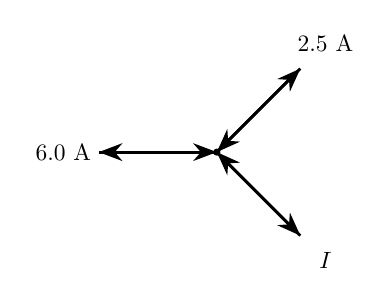
\begin{tikzpicture}[scale=1.0]
  \fill (0,0) circle (1.3pt);
  \jarrow{180}{in}{$6.0$ A}
  \jarrow{45}{out}{$2.5$ A}
  \jarrow{315}{out}{$I$}
\end{tikzpicture}
\end{center}

\worksp{sm}

\prob Three wires carry current \emph{into} the junction shown below:
$1.5$ A, $2.0$ A, and $2.5$ A. One wire carries it all back out. Find that
current.

\begin{center}
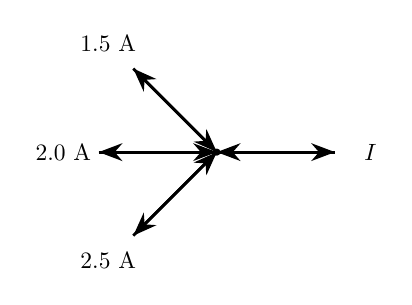
\begin{tikzpicture}[scale=1.0]
  \fill (0,0) circle (1.3pt);
  \jarrow{135}{in}{$1.5$ A}
  \jarrow{180}{in}{$2.0$ A}
  \jarrow{225}{in}{$2.5$ A}
  \jarrow{0}{out}{$I$}
\end{tikzpicture}
\end{center}

\worksp{sm}

\prob A single loop has $\varepsilon=9.0$ V and \emph{three} series
resistors. Voltmeters across two of them read $2.0$ V and $3.0$ V. Find
the reading across the third.

\worksp{sm}

\prob A single loop has $\varepsilon=30$ V and three series resistors.
$\Delta V_1=10$ V and $\Delta V_2=8.0$ V. Find $\Delta V_3$.

\worksp{sm}

\prob Two resistors, $R_1=3.0\ \Omega$ and $R_2=7.0\ \Omega$, are in
series with a battery of $\varepsilon=20$ V. Find the current supplied by
the battery.

\worksp{sm}

\prob Two resistors are in series with a battery of $\varepsilon=15$ V.
$R_1=2.0\ \Omega$, and the current measured in the circuit is $1.5$ A.
Find $R_2$.

\worksp{sm}

\prob Two resistors, $R_1=8.0\ \Omega$ and $R_2=24\ \Omega$, are in
parallel across a battery of $\varepsilon=24$ V. Find the total current
supplied by the battery.

\worksp{sm}

\prob Two resistors, $R_1=5.0\ \Omega$ and $R_2=20\ \Omega$, are in
parallel across a battery. The \emph{total} current from the battery is
measured to be $5.0$ A. Find $\varepsilon$.

\worksp{sm}

\end{document}
